\section{Versuchsziel}

Ziel des Versuchs.

\section{Grundlagen, Vorbereitung}
\subsection{Unterabschnitt}

Gleichungsblock
\begin{align}
	C_\mathrm{n} & = \frac{1}{T}\int \limits_{-\frac{T}{2}}^{\frac{T}{2}}{f(t)e^{-\mathrm{j}n\omega_0t}}dt \nonumber   \\
	    & = \dfrac{A}{T_0} \cdot \left[\dfrac{e^{-\mathrm{j}n\omega_0t}}{-\mathrm{j}n\omega_0t}\right]_{-\dfrac{\tau}{2}}^{\dfrac{\tau} {2}} \nonumber \\
	    & = -\dfrac{A}{\mathrm{j}n\omega_0 T}\cdot \left[e^{-\mathrm{j}n\omega_0 \dfrac{\tau}{2}}-e^{\mathrm{j}n\omega_0 \dfrac{\tau}{2}}\right]
	\intertext{Mit $e^{\mathrm{j}\varphi}=\cos (\varphi)+\mathrm{j} \sin(\varphi)$ kann dieser Term vereinfacht werden:}
	C_\mathrm{n} & = -\dfrac{A}{\mathrm{j}n\omega_0 T}\cdot \left[\cos\left(-n\omega_0 \dfrac{\tau}{2}\right) + \mathrm{j}\sin\left(-n\omega_0 \dfrac{\tau}{2}\right)-\cos\left(-n\omega_0 \dfrac{\tau}{2}\right)-\mathrm{j}\sin\left(-n\omega_0 \dfrac{\tau}{2}\right)\right]
	\intertext{Mit $\cos(x) =\cos(-x)$ und $\sin(-x)=-\sin(x)$ kann weiter vereinfacht werden:}
	C_\mathrm{n} & =-\dfrac{A}{\mathrm{j}n\omega_0 T}\cdot \left[\mathrm{j}\sin\left(-n\omega_0 \dfrac{\tau}{2}\right) + \mathrm{j}\sin\left(-n\omega_0 \dfrac{\tau}{2}\right)\right]  \nonumber \\
	    & = -\dfrac{A}{\mathrm{j}n\omega_0 T}\cdot \left[-2\mathrm{j}\sin\left(n\omega_0 \dfrac{\tau}{2}\right) \right]
	\intertext{Die Kreisfrequenz $\omega_0$ kann ersetzt werden durch $\omega_0=2\pi f_0 = \frac{2 \pi}{T_0}$:}
	C_\mathrm{n} & = \dfrac{A \cdot T}{2n\pi T}\cdot 2 \sin\left(\dfrac{2n\pi \tau}{2T}\right)  \nonumber \\
	    & = \dfrac{A}{n\pi}\cdot \sin\left(n\pi\frac{\tau}{T}\right)
	\intertext{Nach Erweiterung mit $\dfrac{\frac{\tau}{T}}{\frac{\tau}{T}}$}
	C_\mathrm{n} & = \dfrac{A\cdot \tau}{T} \cdot \dfrac{\sin\left(\frac{n\pi \tau}{T}\right)}{\frac{n\pi \tau}{T}}
	\intertext{kann mit der $\mathrm{si}$-Funktion vereinfacht werden:}
	C_\mathrm{n} & = \dfrac{A\cdot \tau}{T} \cdot \mathrm{si}\left({\frac{n\pi \tau}{T}}\right) \label{eq:koeff_si}
\end{align}

\section{Versuchsaufbau, Versuchsdurchführung}
\subsection{Schaltplan und Geräteliste}
Der allgemeine Versuchsaufbau ist nachfolgend in Abbildung \ref{fig:1} dargestellt:

\begin{minipage}[t]{\textwidth-10pt}
	\centering
	\captionsetup{type=figure}
	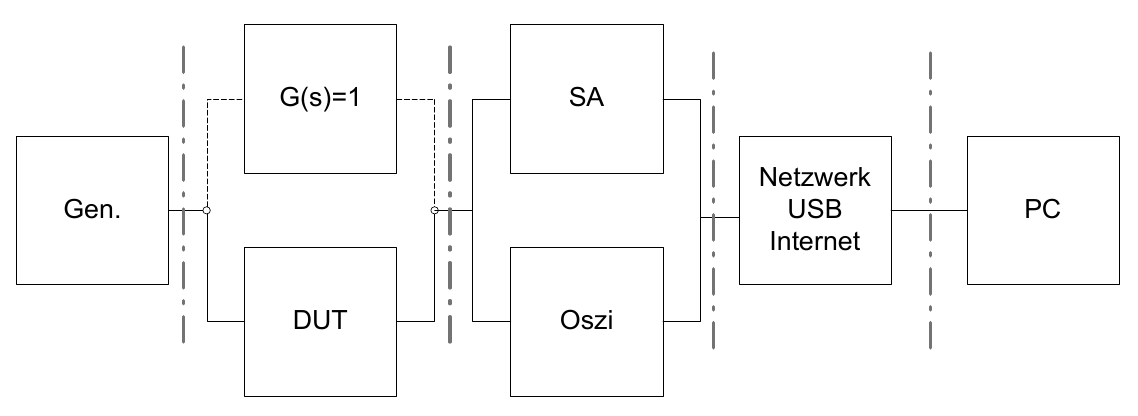
\includegraphics[width=0.9\textwidth]{assets/images/Versuchsschema.png}
	\captionof{figure}{Schematischer Aufbau des Versuchs \cite{oA:2022:bk}}
	\label{fig:1}
\end{minipage}

\subsection{Versuchsdurchführung}

\section{Auswertung}

\newpage
\section{Literaturverzeichnis}
\printbibliography
\newpage

\appendix
\section{Anhang}
\subsection{Messwerte}	
\vspace{0.5cm}
\begin{table}[h]
	\centering
	\captionof{table}{Messwerte, berechnete Fourier-Koeffizienten und Beträge der Übertragungsfunktion}
	\label{tab:mess}
	\begin{tabularx}{\textwidth}{cCCCCCc}
		\toprule
		\makecell{$\pmb{n}$\\$ $\\$ $} 
			& \makecell{$\pmb{U_{e}} /$\\$ \unit{\milli\volt}$ \\ gemessen} 
			& \makecell{$\pmb{U_{a}} /$\\$ \unit{\milli\volt}$ \\ gemessen}
			& \makecell{$\displaystyle \pmb{\frac{U_a}{U_e}}$\\$ $\\}
			& \makecell{$\pmb{U_e} /$\\$\unit{\milli\volt}$ \\ berechnet}
			& \makecell{$\pmb{U_a} / $\\$\unit{\milli\volt}$ \\ berechnet} 
			& \makecell{$\displaystyle \pmb{\frac{U_a}{U_e}} \Big \vert _{U_e=\hat{U}\sin 2 \pi \cdot n f_0}$\\$ $} 
		\\ \midrule
		\csvreader[
			head to column names,
			late after line=\\,
			late after last line=\\ \bottomrule]
			{assets/data/Messwerte.csv}{}{\num{\1} & \num{\2} & \num{\3} & \num{\4} & \num{\5} & \num{\6} & \num{\7}}
	\end{tabularx}
\end{table}